\documentclass[11pt,a4paper]{article}
\usepackage[utf8]{inputenc}
\usepackage[german]{babel}
\usepackage[T1]{fontenc}
\usepackage{amsmath}
\usepackage{amsfonts}
\usepackage{amssymb}
\usepackage{graphicx}
\usepackage{color}
\usepackage[left=2cm,right=2cm,top=2cm,bottom=2cm]{geometry}
\author{Christian Weiß}
\title{Implementierung und Evaluirung eines SNMP Scanners}

\begin{document}

% -----------------------------------------------------------------------------------------------------------------------------------------
% Definitionen
% -----------------------------------------------------------------------------------------------------------------------------------------
\newcommand{\emptyline}{\ \\}

% -----------------------------------------------------------------------------------------------------------------------------------------
% Titelblatt
% -----------------------------------------------------------------------------------------------------------------------------------------
\begin{figure}	% Logo
	\centering
	
\includegraphics[scale=.7]{Bilder/hsa.jpg}
	\label{img:logo}
\end{figure}
	
\vspace{\fill}

\begin{center}
	
	\begin{Huge}
		Abschlussarbeit\linebreak
	\end{Huge}
	
	\vspace{\fill}
	
	\begin{Large}
		Fakultät für Informatik\linebreak
	\end{Large}
	
	\vspace{\fill}
	
	\begin{LARGE}
		Titel\linebreak
	\end{LARGE}
	
	\vspace{1cm}
	
	\begin{Huge}
		\textbf{Implementierung und Evaluation eines SNMP Scanners}\linebreak
	\end{Huge}
	
	\vspace{\fill}
	
	\begin{Large}
		\begin{tabular}{r l}
			Autor: & Christian Weiß \\
			Prüfer: & Prof. Dr. Winter \\
			Datum: & \today \\
		\end{tabular}
	\end{Large}
	
\end{center}	% END - Titleseite
\pagebreak

% -----------------------------------------------------------------------------------------------------------------------------------------
% Inhaltsverzeichnis
% -----------------------------------------------------------------------------------------------------------------------------------------
\tableofcontents

% -----------------------------------------------------------------------------------------------------------------------------------------
% Einleitung (Motivation)
% -----------------------------------------------------------------------------------------------------------------------------------------
%\setcounter{page}{1}
\section{Einleitung}
Das Internet ist ein weltweiter Verbund von Rechnernetzwerken. Physikalisch besteht das Internet im Kernbereich aus einzelnen Netzwerken von Providern, Firmen und Universitäts- und Forschungsnetzwerke. Router verbinden diese Netzwerke miteinander.\\
Das Internet im Ganzen ist unbekannt. Selbst Netzbetreiber kennen nur einen kleinen Teil. Eine Verwaltung findet nur in den Subnetzen statt. Das macht eine Erfassung und Überwachung schwierig. Um den Zustand des Internet zu messen, sind viele Messstellen notwendig. Gut geeignet als Messstellen sind Endgeräte die sich regelmäßig Pakete durchs Internet schicken. Dieser Datenverkehr aus den Messungen kann Aufschluss über das Internet geben. Dafür wurde in der Hochschule eine App namens „Glimpse“ entwickelt, die auf allen erdenklichen Endgeräten installiert werden kann.
Glimpse verfügt über verschiedene Messmethoden, wie z.B. ein Bandbreitentest. Die Endgeräte sollen aus den Subnetzen, in denen sie sich befinden, die Bandbreite des Netzwerks zum Internet messen. Doch das Ergebnis einer solchen Messung kann keinen direkten Aufschluss zur Bandbreite geben. Waren zum Zeitpunkt der Messung noch andere Verbindungen aktive, so kann der gemessene Wert von der Bandbreite des Netzwerks stark Abweichen. Um nun eine bessere Einschätzung machen zu können, müsste man wissen, wie viele Verbindungen während der Messung bestanden haben. Diese Information hält ein Router in seinen Statistiken.\\
Es gibt verschiedene Protokolle mit denen Administratoren ihre Geräte im Netzwerk verwalten können. Darunter fallen Netconf und SNMP (Simple Network Management Protocol). Das Simple Network Management Protocol ist bereits weit verbreitet. Auf vielen Geräten wie Routern, Switches und Druckern ist vom Hersteller die Software bereits installiert. Ausgeliefert werden sie mit Standardpasswörtern, die von den Administratoren oft nicht geändert werden. Das bietet mir die Möglichkeit diese Geräte zu finden und auszulesen.
Findet sich im Subnetz von einem Glimpse-Client ein Gateway-Router, der mit den Standardpasswörtern läuft, können die Statistiken ausgelesen werden.
\pagebreak

% -----------------------------------------------------------------------------------------------------------------------------------------
% Geschichte
% -----------------------------------------------------------------------------------------------------------------------------------------
\section{Geschichte}
„Die Geschichte des SNMP hängt stark mit der Geschichte des Internets zusammen.[…]
So entstand im Jahre 1987 das SGMP (Simple Gateway Monitoring Protocol), da zu damaliger Zeit das Verbinden der Gateways das Hauptproblem war. Gleichzeitig entstand noch ein anderes Protokoll mit dem Namen HEMS (High Level Management Entity System), dessen Entwicklung schon länger zurückreichte. Allerdings fand dieses keine breite Unterstützung im Gegensatz zu dem SGMP, das schon zu dieser Zeit anfing, sich durchzusetzen. Ein weiterer Ansatz lag in einem OSI basierten Protokoll CMIP (Common Management Information Protocol) das auf TCP Protokoll aufgesetzt werden sollte und somit den Namen CMOT erhielt (CMIP over TCP). Aufgrund der geringen Durchsetzung von HEMS wurden nur SGMP und CMOT weiterentwickelt, ersteres, weil es schon weit verbreitet war und zweiteres, weil es auf einem langen ISO-standardisierten Untergrund aufbaute. Später sollten beide zu einem Protokoll verschmelzen.
1988 brachten die Entwickler um SGMP das RFC 1065 Structure of Managment Information [MR88b], RFC 1066 Managment Information Base [MR88a] und RFC 1067 Simple Network Managment Protocol [CFSD88] heraus, was dann 1989 zu recommended erklärt wurde, welches einem quasi-Standard entspricht und ab hier auch schon den Namen SNMP trägt. […]
SNMPv2 war allerdings von seinem Sicherheitsstandard her zu komplex, so dass dies keine breite Zustimmung fand und so wurde 1996 SNMPv2 nur mit dem Sicherheitsmanagement aus SNMPv1 noch mal als RFC eingereicht, was dann SNMPv2c genannt wurde. Doch auch diese Lösung wurde nicht als zufriedenstellend empfunden und so entstanden die beiden Standards SNMPv2u und SNMPv2*, die das Sicherheitsproblem lösen sollten.
Als letztes ist noch SNMPv3, RFC 2272-2275, zu erwähnen, das als Nachfolger von SNMPv2 zu verstehen ist, aber zusätzlich noch die Vereinigung von SNMPv2u und SNMPv2* bewirken soll [Bla97]. Diese wurde 1998 zum Proposed Internet Standard und dann 1999 zum Draft Internet Standard.“
\cite{history}
\pagebreak

% -----------------------------------------------------------------------------------------------------------------------------------------
% Netzwer Management
% -----------------------------------------------------------------------------------------------------------------------------------------
\section{Netzwerk Management}
„Netzwerkmanagement beinhaltet die Installation, Integration und Koordination von Hardware, Software und menschlichen Elemente zum Überwachen, Testen, Abfragen, Konfigurieren, Analysieren, Bewerten und Kontrollieren des Netzwerks und seiner Element-Ressourcen, um die Anforderungen in Bezug auf Performance im Betrieb und Dienstqualität zu angemessenen Kosten zu erfüllen.“
\cite{netmanagement}
\\
Netzwerkmanagement bedeutet, alle managebaren Entitäten zu Verwalten und Überwachen. Bei den Entitäten handelt es sich im wesentlichen um Router, Switches, Drucker und Server. Um diese Geräte veralten zu können muss sich ein Management System Informationen über den Status dieser Geräte im Netzwerk beschaffen können. Damit lassen sich die Information, die übers Netzwerk ausgetauscht werden, in zwei Kategorien einteilen. Es werden Nachrichten versandt, die über den Status einer Resource informieren und das Management System muss Kommandos an die Ressourcen senden können. Die Nachrichten über den Status können vom Management System angefordert sein, können aber auch vom Gerät selbst als Warnung bei einer Fehlfunktion verschickt werden. Das Management System kann mit Kommandos an Entitäten reagieren um einer Fehlfunktion entgegen zu wirken.
Die folgende Abbildung zeigt eine allgemeine Darstellung einer Netzwerkmanagementarchitektur mit ihren Hauptkomponenten. Die verwaltende Einheit als Rechner oder Notebook (NMS) und verwaltete Geräte mit ihren Agenten (A).
\\
\begin{figure}[h]
	\centering
	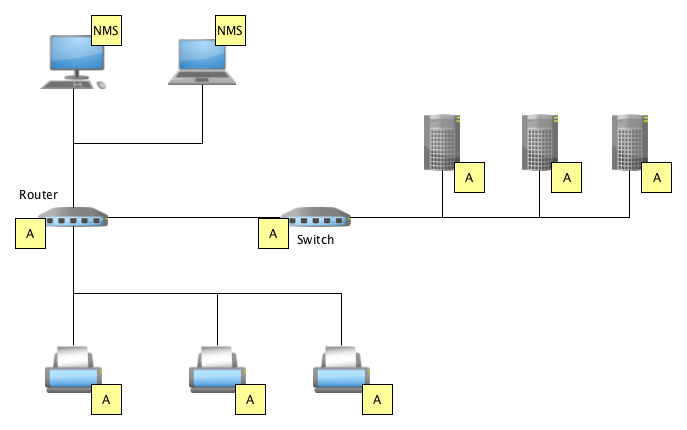
\includegraphics[scale=.5]{Bilder/Netzwerk.png}
	\caption{Beispiel Netzwerk mit allen Entitäten.}
\end{figure}

% -----------------------------------------------------------------------------------------------------------------------------------------
% Netzwerk Management System
% -----------------------------------------------------------------------------------------------------------------------------------------
\section{Network Management Station}
Eine NMS ist ein Rechner der im selben Netzwerk angesiedelt ist wie die Agenten mit denen es kommuniziert. Auf diesem Rechner läuft eine Software, die dem Administrator das Überwachen und Konfigurieren seiner Geräte im Netzwerk erlaubt. Eine NMS kann auch automatisiert sein und auf Fehlermeldungen der Agenten reagieren.
\\

% -----------------------------------------------------------------------------------------------------------------------------------------
% Agent
% -----------------------------------------------------------------------------------------------------------------------------------------
\section{Agenten}
Ein Agent ist ein Softwaremodul, dass auf einem netzwerkfähigem Gerät installiert ist. Diese Software bildet die Schnittstelle zwischen dem Gerät und dem Managementsystem. Ein NMS kann einen Request an den Agenten senden um den Status einer Resource zu erfragen. Der Agent liest die angeforderten Informationen aus seinem Wirt aus. Diese Informationen packt der Agent in einen RequestResponse und antwortet damit dem NMS. Die Eigenschaften eines Gerätes, welches von einem Agenten verwaltet wird, können vom NMS auch verändert werden. Zu den Informationen, die der Agent überwacht und übermitteln kann, gehören Konfigurationsdaten, Statusinformationen und Statistikwerte.
Kritische Eigenschaften eines Gerätes können vom Agent permanent überwacht werden. Triftet ein Wert einer Überwachten Eigenschaft in einen kritischen Bereich ab, kann das der Agent registrieren. Er reagiert sofort und sendet eine Warnung an das NMS.
Jeder Agent hat dazu eine Management Information Base (MIB) in der die Werte spezifiziert sind, die er verwalten und überwachen kann. Die Einträge in der MIB verweisen auf die Managed Objects vom Gerät.
\\
\begin{figure}[h]
	\centering
	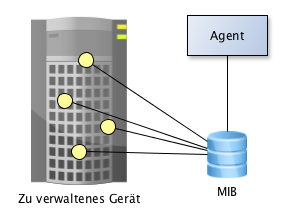
\includegraphics[scale=.7]{Bilder/Agent.png}
	\caption{EIn Agent und seine Managed Objects aus der MIB}
\end{figure}

% -----------------------------------------------------------------------------------------------------------------------------------------
% Agent
% -----------------------------------------------------------------------------------------------------------------------------------------
\section{Management Information Base (MIB)}
Die Management Information Base (MIB) enthält alle Managed Objects, die ein Agent später referenzierten kann. Die einzelnen Objekte müssen in der MIB detailliert beschrieben werden. Jedes Object erhält seine eigenen Zugriffsrechte, die später für die Anfragen von einem NMS an den Agenten gelten sollen. Damit durch ein NMS gezielt solche Objekte angesprochen werden können, erhalten die Managed Objects eine eindeutige Object ID (OID). Zudem sind zu bestimmen mit welchem Datentype der Status des Objekts anzugeben ist und es es gibt eine Beschreibung für das Objekt in Textform.\\
Die Module und Objekte einer MIB sind angeordnet in Baumform und können mit der OID referenziert werden. Ein Identifier zu einem Managed Object im Baum besteht aus Nummern und kann z.B. so aussehen: „.1.3.6.1.2.1.1“. Die Länge der OID bestimmt die Tiefe im Baum. Eine einzelne Nummer gibt Auskunft über das Blatt auf horizontaler Ebene. Die Blätter tragen auch Namen. So kann eine OID auch wie folgt beschrieben werden: „.iso.org.dod.mgmt.mib-2.system.sysDescr.0“.\\
Die Managed Objects einer MIB werden in der Syntax, die von der SMI vorgegeben wird, in einer ASCII-Datei abgelegt. Diese Datei kann von einem MIB-Compiler für die Verwendung durch einen Agenten aufbereitet werden.
\\
\begin{figure}[h]
	\centering
	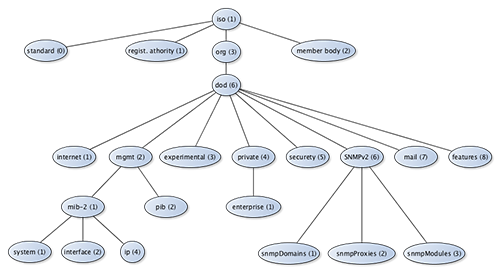
\includegraphics[scale=1]{Bilder/MIB.png}
	\caption{Die grobe Struktur des MIB-Baumes}
\end{figure}

% -----------------------------------------------------------------------------------------------------------------------------------------
% Structure of Management Information SMI
% -----------------------------------------------------------------------------------------------------------------------------------------
\section{Structure of Management Information (SMI)}
Die SMI ist eine Sprache zur Beschreibung der MIB’s und wurde für SNMP entwickelt. Damit lassen sich die Module, Managed Objects und Notifications für die MIB erstellen. Die SMI legt dazu die Syntax fest, mit der eine MIB beschrieben werden kann. Außerdem sind verschiedene Datentypen wie INTEGER, Gauge, Counter64 und viele mehr definiert. Ansonsten ist die SMI ein Auszug aus der ASN.1.
Ein Beispiel für einen MIB-Eintrag in der Form, wie sie von der SMI vorgegeben wird:
\\
\begin{figure}[h]
	\centering
	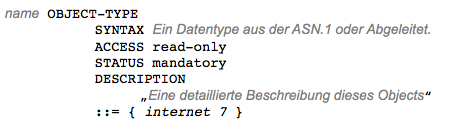
\includegraphics[scale=1]{Bilder/mibEintragSMI}
	\caption{Ein Eintrag in der MIB geschrieben mit den Vorgaben aus der SMI}
\end{figure}
Damit würde ein Eintrag im Baum entstehen, der  wie folgt zu erreichen ist: iso.org.dod.internet.neuesObj\\
und als Object Identifier : 1.3.6.1.7.0

% -----------------------------------------------------------------------------------------------------------------------------------------
% Abstract Syntax Notation One ASN.1
% -----------------------------------------------------------------------------------------------------------------------------------------
\section{Abstract Syntax Notation One (ASN.1)}
Zwischen den verschiedenen Geräten im Netzwerk kann es zu Inkompatibilitäten kommen. Die Hardware oder auch die installierte Software kann für die Daten unterschiedliche Darstellungen verwenden. Ein Beispiel dafür ware Big Endian und Little Endian. Bei der Kommunikation mit SNMP zwischen den Agenten und dem NMS müssen die Daten jedoch klar definiert sein. SNMP setzt für die Kompatibilität auf eine Teilmenge der ASN.1.\\
Die ASN.1 bietet einen Standard zur Definition von Datentypen und deren Werte. Ein Datentype ist eine Art von Information. Eine Information kann Beispielsweise eine Zahl, ein Text, ein Bilde oder auch ein Video sein. Für diese Informationen sollen Datentypen bereitgestellt werden. Ein Wert hingegen ist eine Instanz von einem dieser Datentypen. In der ASN.1 sind verschiede primitive Datentypen und deren Werte beschrieben. Außerdem finden sich Regeln um einfache Datentypen zu kombinieren, wodurch man komplexere Typen erzeugt. Es ist ein Werkzeugkasten um Daten in eine bestimmte  Form zu bringen.
\\

% -----------------------------------------------------------------------------------------------------------------------------------------
% Basic Encoding Rules BER
% -----------------------------------------------------------------------------------------------------------------------------------------
\section{Basic Encoding Rules (BER)}
Bei der Übertragung von Daten durch ein Netzwerk muss der Empfänger die Daten interpretieren können. Dafür ist immer ein Standard wie zum Beispiel ein Protokoll nötig. Die Basic Encoding Rules sind eines von drei Standards der ASN.1 zum Codieren der Daten. In dieser Codierung beschreiben und limitieren sich die Daten selbst. Die Daten werden mit einer Angabe über den Datentype und einer Angabe der die Länge in Bytes versehen. Gefolgt von den Daten selbst. Diese Vorgehensweise wird auch TLV-Encoding genannt. In einem eingehendem Datenstrom können Daten, die so codiert wurden, vom Empfänger leicht interpretiert werden. Der Empfänger muss noch nicht einmal die gesamte Nachricht erhalten, um einzelne Daten lesen zu können.
\\
\begin{figure}[h]
	\centering
	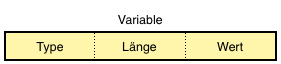
\includegraphics[scale=1]{Bilder/BasicEncodingRules}
	\caption{Darstellung eines Wertes in den Basic Encoding Rules}
\end{figure}

\subsection{Der Type}
Der Datentype wird normalerweise mit einem Byte bestimmt. Doch von diesem Byte sind die 3 höchsten Bit reserviert. So kann es vorkommen, dass der Datentype mit mehreren Bytes beschrieben wird. Mit fünf Bits können nur 31 verschiedene Typen definiert werden.
\\
\begin{figure}[h]
	\centering
	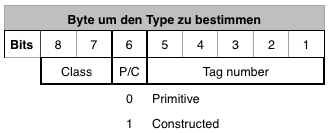
\includegraphics[scale=1]{Bilder/Datentype-BER}
	\caption{Die Verwendung der einzelnen Bits im Byte Datentype}
\end{figure}

Man unterscheidet zwischen komplexen und primitiven Datentypen. Primitive Typen sind einfache Datentypen wie zum Beispiel Integer. Komplexe Datentype sind Konstrukte bestehen aus mehreren einfachen Datentypen. Welcher Art das Datum ist, steht in Bit 6.
\\
Die Datentypen lassen sich außerdem in vier Klassen einteilen. Die Klassen sind Universal, Application, Context-specific und Private. Sie werden in den beiden höchsten Bits 7 und 8 dargestellt.
\\
\begin{figure}[h]
	\centering
	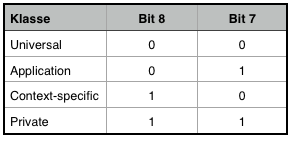
\includegraphics[scale=1]{Bilder/datentypeKlassen}
	\caption{Die verschiedenen Klassen der Datentypen}
\end{figure}

\subsection{Die Länge}
Die Länge des Datums kann in drei verschiedenen Varianten auftreten. Sie kann in kurzer oder in langer Form angegeben werden. Beide sind definit. Die dritte Form is indefinit. Es wird keine Länge angegeben.

\subsubsection{Kurze definite Form}
Die einfachste Form, mit der die Länge eines Datums bestimmt wird, ist definit und ein Byte lang. Dazu muss in diesem Byte das höchste Bit 0 sein. In den restlichen 7 Bits kann die Länge des Datums in Bytes eingetragen werden. Dadurch, dass das höchste Bit 0 sein muss, liegt der Wertebereich nur bei 0 - 127 Bytes. Diese Notation ist also nur für Daten geeignet, die nicht länger als 127 Bytes sind.
\\
\begin{figure}[h]
	\centering
	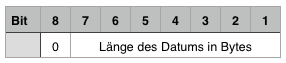
\includegraphics[scale=1]{Bilder/laengeDefinitKurz}
	\caption{Die Länge des Datums in kurzer definiter Form}
\end{figure}

\subsubsection{Lange definite Form}
Die lange definite Form der Längenangabe erstreckt sich über mehrere Bytes. So können sehr große Werte eingetragen werde. Dazu muss das erste Byte signalisieren, das sich die Längenangabe mehrere Bytes lang ist. Deshalb in diesem Byte das höchste Bit auf 1 gesetzt werden. Die Bits 7-1 geben auskunft über die Anzahl der Bytes, die folgen. Für einen 16 Bit Integer würden zum Beispiel zwei Bytes folgen. Eingetragen werden sie beginnen mit dem höchsten Byte.
\\
\begin{figure}[h]
	\centering
	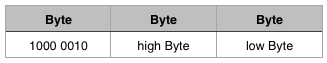
\includegraphics[scale=1]{Bilder/laengeDefinitLang}
	\caption{Die Länge des Datums in langer definiter Form}
\end{figure}

\subsubsection{Länge indefinit}
In der indefiniten Form wird keine Angabe über die Länge des Datums gemacht. Das Byte für die Längenangabe hat das höchste Bit auf eins gesetzt, was bedeuten würde, dass weitere Bytes für die Längenangabe folgen. Doch die Anzahl der folgenden Bytes wird mit 0 angegeben. Nun ist die Länge des Datums ungewiss. Die Bytes des Datums werden eingetragen. Da die Länge jedoch nicht bestimmt wurde, muss das Ende des Datums markiert werden. Eine "end-of-contents" Marke muss angehängt werden. Die "end-ofcontents" Marke besteht aus zwei leeren Bytes.
\\
\begin{figure}[h]
	\centering
	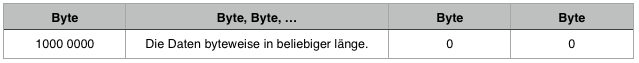
\includegraphics[scale=.75]{Bilder/laengeIndefinit}
	\caption{Die Länge in indefiniter Form}
\end{figure}

\subsection{Das Datum}
Das Datum selbst wird byteweise eingetragen, wobei mit dem höchsten Byte begonnen wird. Das niederste Byte komm zuletzt. Die Anzahl der Bytes muss mit der Längenangabe übereinstimmen.
\\

% -----------------------------------------------------------------------------------------------------------------------------------------
% Das SNMP Protokoll
% -----------------------------------------------------------------------------------------------------------------------------------------
\section{Das SNMP Protokoll}
SNMP steht für Simple Network Management Protocol. Es wurde entwickelt für die Kommunikation zwischen verschiedenen Geräten und einem NMS im Netzwerk.\\
\emptyline
Das mit diesem Protokoll angestrebte Ziel beschreiben die Entwickler wie folgt:\\
„The SNMP explicitly minimizes the number and complexity of management functions realized by the management agent itself.  This goal is attractive in at least four respects:\\
      (1)  The development cost for management agent software necessary to support the protocol is 	accordingly reduced.\\
      (2)  The degree of management function that is remotely supported is accordingly increased, 	thereby admitting fullest use of internet resources in the management task.\\
      (3)  The degree of management function that is remotely supported is accordingly increased, 	thereby imposing the fewest possible restrictions on the form and sophistication of 		management tools.\\
      (4)  Simplified sets of management functions are easily understood and used by developers of 	network management tools.\\
\emptyline
A second goal of the protocol is that the functional paradigm for monitoring and control be sufficiently extensible to accommodate additional, possibly unanticipated aspects of network operation and management.\\
\emptyline
A third goal is that the architecture be, as much as possible, independent of the architecture and mechanisms of particular hosts or particular gateways.“
\cite{rfcSnmpGoals}\\
\emptyline
Vom SNMP Protokoll gibt es heute mehrere Versionen. Die erste Version vom Protokoll hatte kaum Sicherheitsmechanismen. Es wurde zu unsicher. Deshalb haben die Entwickler neue Entwürfe heraus gebracht. Die Version 2 von SNMP gibt es in mehreren Ausführungen mit verschiedenen Ansätzen zur Schliessung der Sicherheitslücken. Doch die Umsetzung der Versionen SNMPv2u und SNMPv2p waren den meisten Anwendern zu umständlich, sie fanden kaum Akzeptanz. SNMPv2* wurde erst gar nicht veröffentlicht. Letztendlich verzichtete man auf die Sicherheitsmechanismen und brachte die Version SNMPv2c hervor. Damit wurde die erste Version mit neuen Features der der zweiten Version erweitert. Um dem Verlangen nach Sicherheit doch noch gerächt zu werden, haben die Entwickler noch eine dritte Version aufgelegt, SNMPv3.\\
Die Architektur besteht aus zwei einfachen Elementen, den Managern und den Agenten. Die Manager werden meist als Network Management Station (NMS) bezeichnet. Die Manager stellen Anfragen an die Agenten um Informationen über deren Gerät im Netzwerk zu erhalten. Sie können aber auch Änderungen an den Einstellungen eines Gerätes vornehmen. So ermöglicht es dem Administrator das zentrale Verwalten seiner Geräte im Netzwerk.
SNMP ermöglicht die Überwachung von Netzwerkkomponenten, bietet eineFernkonfiguration und Fernsteuerung von Netzwerkkomponenten an. Außerdem gibt es eine Fehlererkennung mit Benachrichtigung. Agenten überwachen sich selbst. Stellen sie eine Fehlfunktion fest, senden sie eine Notifikation an ihre Management Station.\\
SNMP kann mit verschiedenen Transportprotokollen verwendet werden. Meistens werden die SNMP Pakete jedoch mit UDP versandt.
Mit SNMP werden Anfragen an ein Gerät im Netzwerk gestellt. Diese Anfragen (Request) können vom Gerät einen Wert als Antwort anfordern. Sie können das Gerät aber auch auffordern einen Wert in dessen Einstellungen zu ändern.\\
Wenn ein Request einen Fehler aufweist, also nicht dem Protokoll entspricht, dann ist vom Agent keine Antwort zu erwarten.\\
Zur Übertragung der Daten werden in allen Versionen die BER verwendet. Das gesamte Paket wird in dieser Form der Codierung geschrieben.
\\

% -----------------------------------------------------------------------------------------------------------------------------------------
% Literaturverzeichnis
% -----------------------------------------------------------------------------------------------------------------------------------------
\section{Protokollaufbau}
\subsection{SNMPv1}
\begin{figure}[h]
	\centering
	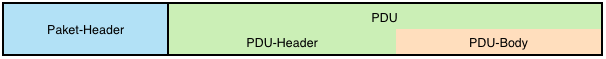
\includegraphics[scale=1]{Bilder/SNMPv1-Aufbau}
	\caption{Der Protokollaufbau von SNMP Version 1}
\end{figure}
Das Paket unterteilt sich im im wesentlichen in zwei Teile. Der Header und die Protocol Data Unit (PDU). Der Header gibt Auskunft über die Länge des gesamten Pakets, die verwendete Protokoll Version und einen Community-Namen. In der PDU sind die zu übertragenden Daten enthalten, sowie eine Fehlermeldung.\\

\subsubsection{Header}
\begin{figure}[h]
	\centering
	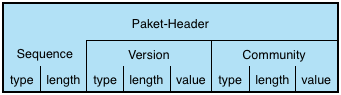
\includegraphics[scale=1]{Bilder/SNMPv1-Header}
	\caption{Der Header von SNMP Version 1}
\end{figure}
Der Inhalt eine SNMP Nachricht besteht aus einer Ansammlung von Daten, einer Sequenz. Der Header beginnt deshalb mit dem ASN.1 Datentype „Sequence“. Die Länge entspricht dem gesamten Paket in Bytes. Der rest des Paketes entspricht dem Wert in diesem TLV-Encoding.
Die Version die Version des Protokolls, die verwendet wird, ist vom Datentype INTEGER. Für die Länge ist hier nur ein Byte ausreichend. Die Versionsnummer sind fortlaufend durchnummeriert, beginnend bei 0 mit SNMPv1.\\
Die Community dient hier der Sicherheit und ist als eine Art Passwort gedacht. Es gibt ein solches „Passwort“ jeweils fürs Auslesen von Daten und zum Editieren von Konfigurationen an den Geräten. Vom Hersteller werden meist „public“ zum lesen und „private“ zum schreiben voreingestellt. Als Datentype verwendet man üblicherweise OCTED STRING. Für jedes Zeichen wird ein Byte verwendet.\\

\subsubsection{Protocol Data Unit (PDU)}
\begin{figure}[h]
	\centering
	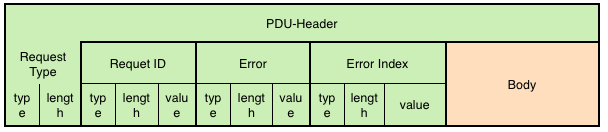
\includegraphics[scale=1]{Bilder/SNMPv1-PDU}
	\caption{Die PDU von SNMP Version 1}
\end{figure}
Die PDU hat selbst auch einen Header. Im header wird der Request Type angegeben. Der Request Type ist vom Type IMPLICIT SEQUENCE. Die Typen geben den Zweck der Nachricht an. Zum Auslesen von Konfigurationsdaten sendet man „GetRequest“ oder „GetNextRequest“. Um die Konfiguration an einem Gerät zu ändern, sendet man einen „SetRequest“. Die Geräte antworten mit einem „RequestResponse“. Stellt ein Agent ungewöhnliche Werte an Gerät fest, sendet er eine „Trap“ Nachricht. Als Länge trägt man hier die gesamt Länge der PDU ein. Der rest der PDU entspricht dem Wert im TLV.\\
Außerdem enthält der Header eine Request ID, einen Fehlerwert und die Position des Fehlers. Jeder dieser Werte wird als TLV eingetragen.
Die Request ID ist ein beliebiger zahlen Wert, der die Nachricht eindeutig identifiziert.
Das Error-Feld kann einen von 0 verschiedenen Wert nur dann haben, wenn es sich um eine Antwort oder Benachrichtigung von einem Agent handelt. Mögliche Fehlermeldungen sind:\\
\begin{figure}[h]
	\centering
	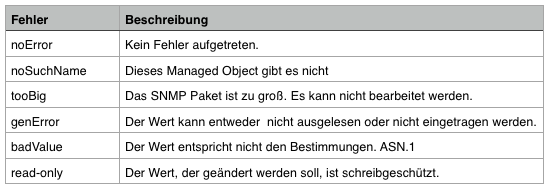
\includegraphics[scale=1]{Bilder/SNMPv1-Fehler}
\end{figure}
In einem SNMP Paket können mehrere Werte abgefragt werden. Dann enthält der PDU-Body mehrere Variablen Bindings. Wenn eine dieser Variablen einen Fehler verursacht, ist die Position dieser Variablen im Feld Error Index hinterlegt.\\

\subsubsection{PDU - Body}
\begin{figure}[h]
	\centering
	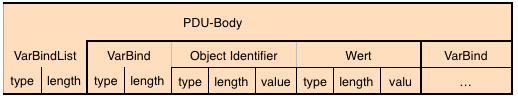
\includegraphics[scale=1]{Bilder/SNMPv1-PDU-Body}
	\caption{Der Body aus der PDU. Der Teil mit den Variablen.}
\end{figure}
Im PDU-Body werden die Werte übertragen. Eine oder mehrere Variablen können in der „VarBindList“ zusammen gefasst werden. Auch hier wird alles TLV-Codiert. Diese Liste der Variablen ist vom Type SEQUENCE. Die einzelnen Variablen bestehen aus einer OID und dem zugehörigem Wert selbst. Die beiden werden ebenso überspannt von einer SEQUENCE, dem „VarBind“.\\
Der Object Identifier und der dazu gehörigeWert werden ebenfalls im TLV-Encoding eingetragen. Bei einer Anfrage wird nur die OID und kein Wert übertragen, den soll der Agent zurücksenden. Für diesem Fall gibt es den Datentype NULL. Die Länge wird auch auf 0 gesetzt und Daten im Feld ‚value‘ werden keine eingetragen.\\

\subsubsection{Veränderter Header bei Traps}
Ein Agent kann Teile des System auf dem er läuft selbstständig überwachen, so muss des Management System nicht permanent den Status abfragen. Der Agent kann konfiguriert werden auf bestimmte Werte ein Auge zu haben. Wenn eine dieser Systemeigenschaften eine kritische Marke über- oder unterschreitet, dann sendet der Agent eine Warnung an den Manager. Diese Art von Benachrichtigungen nennt man Traps. Für diese Traps gibt es einen eigenen PDU-Header.\\
\begin{figure}[h]
	\centering
	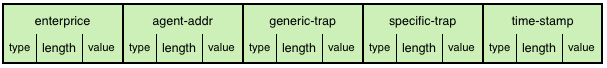
\includegraphics[scale=1]{Bilder/SNMPv1-Header-Traps}
	\caption{Die Unterschiede im Header bei Traps}
\end{figure}
Gleich nach dem PDU Type folgt das Feld ‚enterprice‘. Im Feld ‚enterprise‘ ist immer ein Object Identifier zu finden. Er identifiziert die Eigenschaft, deren Wert für diese Warnung sorgte. Der Agent , der diese Nachricht versendet trägt seine IP-Adresse im Feld ‚agent-addr‘ ein. Der Datentype dafür ist festgelegt als NetworkAddress.\\
Das Feld ‚generic-trap‘ enthält einen Integer und kann folgende vordefinierte Fehler enthalten :\\
\begin{figure}[h]
	\centering
	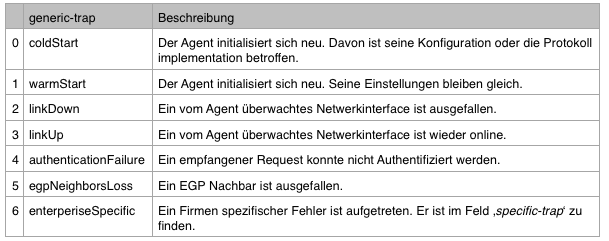
\includegraphics[scale=1]{Bilder/SNMPv1-Traps-Fehler}
\end{figure}
Das Feld ‚specific-trap‘ wird nur gebraucht, wenn der Fehler nicht einer der generischen Fehlertypen ist. Der Datentype ist als Integer festgelegt. Hier können vom Hersteller oder vom Administrator eigene Fehlertypen eingetragen werden.\\
Im letzten Feld übermittelt der Agent die Zeit, die seit seinem letzten Neustart vergangen ist. Der Zeitstempel wird angegeben mit dem Datentype TimeTicks.\\

% -------------
\pagebreak
% -----------------------------------------------------------------------------------------------------------------------------------------
% Literaturverzeichnis
% -----------------------------------------------------------------------------------------------------------------------------------------
\begin{thebibliography}{10}
	\bibitem{history}			% Geschichte
	\begin{small}
		www-i4.informatik.rwth-aachen.de/content/teaching/proseminars/sub/2003\_ss\_proseminar\_docs/snmp.pdf
	\end{small}
	\bibitem{netmanagement}	% Netzwerk Management
		Kurose, J. F.,
		Computernetze: Ein Top-Down-Ansatz mit Schwerpunkt Internet,
		Addison-Wesley,
		2002
	\bibitem{rfcSnmpGoals}
		RFC 1157, Goals of the Architecture, Seite 5
\end{thebibliography}

\end{document}